\section{Geom\-PQP2D  Class Reference}
\label{class_GeomPQP2D}\index{GeomPQP2D@{Geom\-PQP2D}}
A parent class for 2D PQP geometries. 


{\tt \#include $<$geom\-PQP.h$>$}

Inheritance diagram for Geom\-PQP2D::\begin{figure}[H]
\begin{center}
\leavevmode
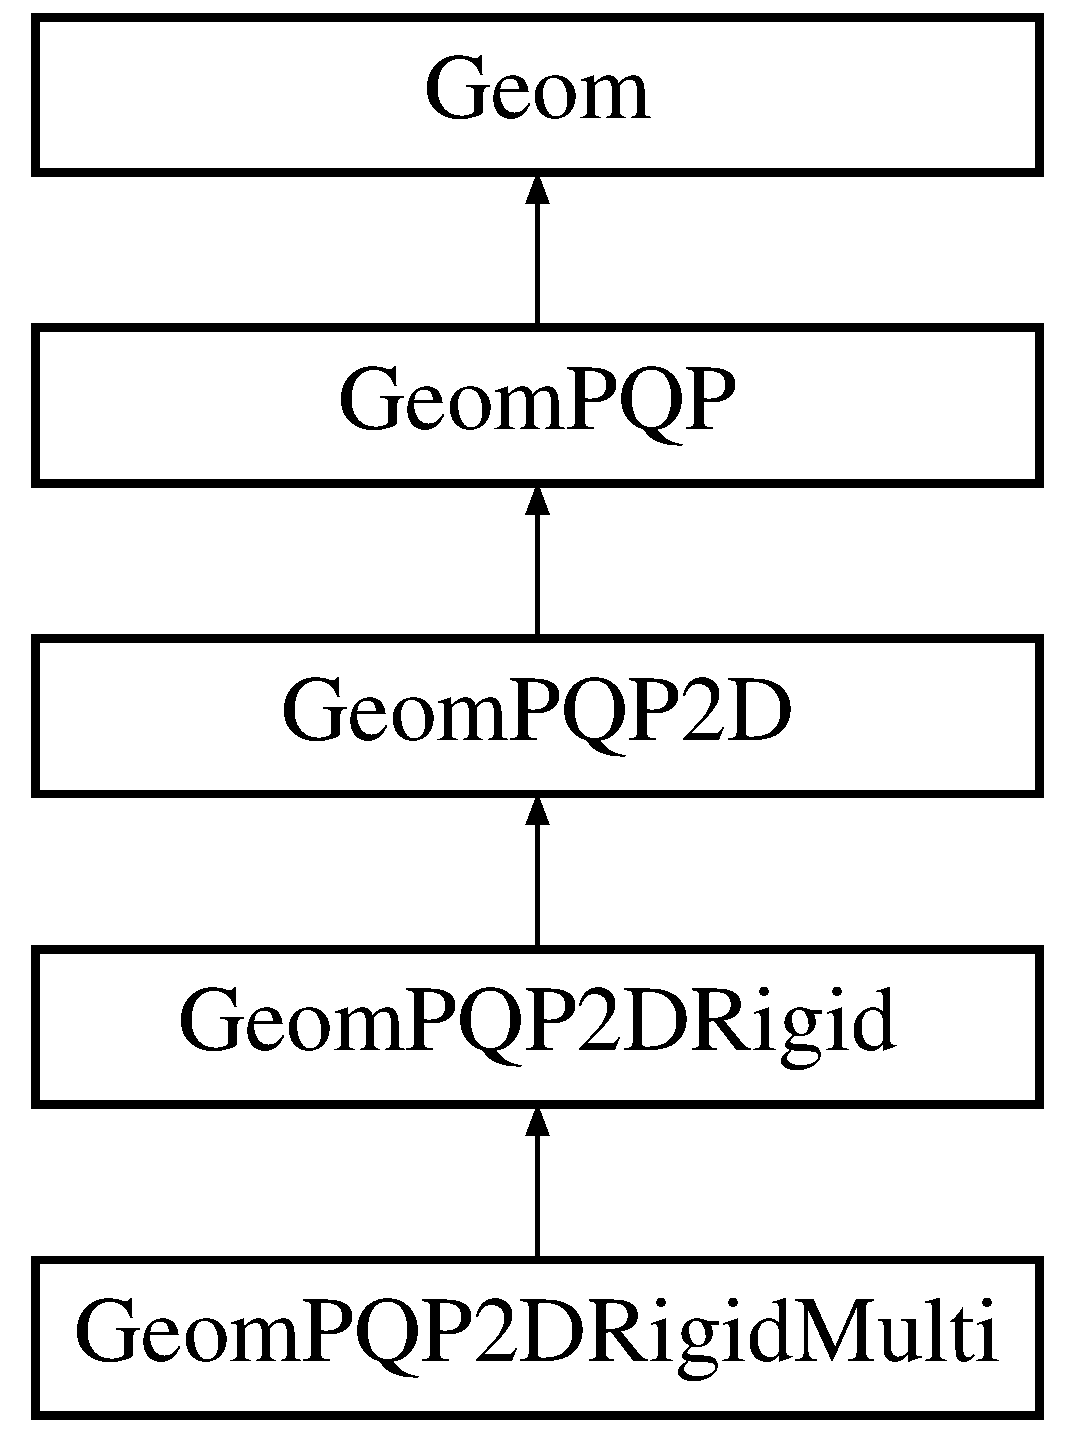
\includegraphics[height=5cm]{class_GeomPQP2D}
\end{center}
\end{figure}
\subsection*{Public Methods}
\begin{CompactItemize}
\item 
{\bf Geom\-PQP2D} (string path)
\item 
virtual {\bf $\sim$Geom\-PQP2D} ()
\item 
virtual void {\bf Load\-Environment} (string path)
\item 
virtual void {\bf Load\-Robot} (string path)
\end{CompactItemize}
\subsection*{Public Attributes}
\begin{CompactItemize}
\item 
list$<${\bf MSLPolygon}$>$ {\bf Obst\-Polygons}
\item 
list$<${\bf MSLPolygon}$>$ {\bf Robot\-Polygons}
\end{CompactItemize}


\subsection{Detailed Description}
A parent class for 2D PQP geometries.



\subsection{Constructor \& Destructor Documentation}
\index{GeomPQP2D@{Geom\-PQP2D}!GeomPQP2D@{GeomPQP2D}}
\index{GeomPQP2D@{GeomPQP2D}!GeomPQP2D@{Geom\-PQP2D}}
\subsubsection{\setlength{\rightskip}{0pt plus 5cm}Geom\-PQP2D::Geom\-PQP2D (string {\em path})}\label{class_GeomPQP2D_a0}


\index{GeomPQP2D@{Geom\-PQP2D}!~GeomPQP2D@{$\sim$GeomPQP2D}}
\index{~GeomPQP2D@{$\sim$GeomPQP2D}!GeomPQP2D@{Geom\-PQP2D}}
\subsubsection{\setlength{\rightskip}{0pt plus 5cm}Geom\-PQP2D::$\sim$Geom\-PQP2D ()\hspace{0.3cm}{\tt  [inline, virtual]}}\label{class_GeomPQP2D_a1}




\subsection{Member Function Documentation}
\index{GeomPQP2D@{Geom\-PQP2D}!LoadEnvironment@{LoadEnvironment}}
\index{LoadEnvironment@{LoadEnvironment}!GeomPQP2D@{Geom\-PQP2D}}
\subsubsection{\setlength{\rightskip}{0pt plus 5cm}virtual void Geom\-PQP2D::Load\-Environment (string {\em path})\hspace{0.3cm}{\tt  [virtual]}}\label{class_GeomPQP2D_a2}




Reimplemented from {\bf Geom\-PQP} {\rm (p.\,\pageref{class_GeomPQP_a2})}.\index{GeomPQP2D@{Geom\-PQP2D}!LoadRobot@{LoadRobot}}
\index{LoadRobot@{LoadRobot}!GeomPQP2D@{Geom\-PQP2D}}
\subsubsection{\setlength{\rightskip}{0pt plus 5cm}virtual void Geom\-PQP2D::Load\-Robot (string {\em path})\hspace{0.3cm}{\tt  [virtual]}}\label{class_GeomPQP2D_a3}




Reimplemented from {\bf Geom\-PQP} {\rm (p.\,\pageref{class_GeomPQP_a3})}.

Reimplemented in {\bf Geom\-PQP2DRigid\-Multi} {\rm (p.\,\pageref{class_GeomPQP2DRigidMulti_a4})}.

\subsection{Member Data Documentation}
\index{GeomPQP2D@{Geom\-PQP2D}!ObstPolygons@{ObstPolygons}}
\index{ObstPolygons@{ObstPolygons}!GeomPQP2D@{Geom\-PQP2D}}
\subsubsection{\setlength{\rightskip}{0pt plus 5cm}list$<${\bf MSLPolygon}$>$ Geom\-PQP2D::Obst\-Polygons}\label{class_GeomPQP2D_m0}


\index{GeomPQP2D@{Geom\-PQP2D}!RobotPolygons@{RobotPolygons}}
\index{RobotPolygons@{RobotPolygons}!GeomPQP2D@{Geom\-PQP2D}}
\subsubsection{\setlength{\rightskip}{0pt plus 5cm}list$<${\bf MSLPolygon}$>$ Geom\-PQP2D::Robot\-Polygons}\label{class_GeomPQP2D_m1}




The documentation for this class was generated from the following file:\begin{CompactItemize}
\item 
{\bf geom\-PQP.h}\end{CompactItemize}
